\documentclass{article}
\usepackage{tikz}
\usepackage{graphicx}  % For including external images
\usepackage{standalone}  % For including standalone files
\usepackage{youngtab}  % For tables
\usepackage{array}  % For \extrarowheight support

\begin{document}
\noindent Here are some samples.\\

%1-3 vertices
\begin{tabular}{|c|c|c|c|}
\hline
\documentclass{standalone}
\usepackage{tikz}
\begin{document}
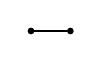
\begin{tikzpicture}[every node/.style={draw, circle, fill=black, minimum size=2pt, inner sep=0pt}]
\node[fill=black] (G1N0) at (6.50,4.50) {};
\node[fill=black] (G1N1) at (7.00,4.50) {};
\draw (G1N0) -- (G1N1);
\end{tikzpicture}
\end{document}
 & \documentclass{standalone}
\usepackage{tikz}
\begin{document}
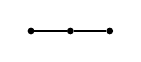
\begin{tikzpicture}[every node/.style={draw, circle, fill=black, minimum size=2pt, inner sep=0pt}]
\node[fill=black] (G1N1) at (5.99,4.51) {};
\node[fill=black] (G1N0) at (6.49,4.51) {};
\node[fill=black] (G1N2) at (6.99,4.51) {};
\draw (G1N0) -- (G1N1);
\draw (G1N0) -- (G1N2);
\end{tikzpicture}
\end{document}
 & \documentclass{standalone}
\usepackage{tikz}
\begin{document}
\begin{tikzpicture}[every node/.style={draw, circle, fill=black, minimum size=2pt, inner sep=0pt}]
\node[fill=black] (G1N1) at (6.00,4.50) {};
\node[fill=black] (G1N0) at (6.50,4.50) {};
\node[fill=black] (G1N2) at (7.00,4.50) {};
\node[fill=black] (G1N3) at (6.50,4.99) {};
\draw (G1N0) -- (G1N1);
\draw (G1N0) -- (G1N2);
\draw (G1N0) -- (G1N3);
\end{tikzpicture}
\end{document}
 & \documentclass{standalone}
\usepackage{tikz}
\begin{document}
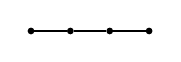
\begin{tikzpicture}[every node/.style={draw, circle, fill=black, minimum size=2pt, inner sep=0pt}]
\node[fill=black] (G1N2) at (6.00,4.50) {};
\node[fill=black] (G1N0) at (6.50,4.50) {};
\node[fill=black] (G1N1) at (7.00,4.50) {};
\node[fill=black] (G1N3) at (7.50,4.50) {};
\draw (G1N0) -- (G1N1);
\draw (G1N0) -- (G1N2);
\draw (G1N1) -- (G1N3);
\end{tikzpicture}
\end{document}
\\  
\hline
\end{tabular}

\vspace{15pt}
%4 vertices
\begin{tabular}{|c|c|c|c|}
    \hline
    \documentclass{standalone}
\usepackage{tikz}
\begin{document}
\begin{tikzpicture}[every node/.style={draw, circle, fill=black, minimum size=2pt, inner sep=0pt}]
\node[fill=black] (G1N1) at (6.00,4.51) {};
\node[fill=black] (G1N0) at (6.50,4.51) {};
\node[fill=black] (G1N2) at (7.00,4.51) {};
\node[fill=black] (G1N3) at (6.50,4.01) {};
\node[fill=black] (G1N4) at (6.50,5.00) {};
\draw (G1N0) -- (G1N1);
\draw (G1N0) -- (G1N2);
\draw (G1N0) -- (G1N3);
\draw (G1N0) -- (G1N4);
\end{tikzpicture}
\end{document}
 & \documentclass{standalone}
\usepackage{tikz}
\begin{document}
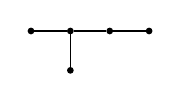
\begin{tikzpicture}[every node/.style={draw, circle, fill=black, minimum size=2pt, inner sep=0pt}]
\node[fill=black] (G1N2) at (6.00,4.50) {};
\node[fill=black] (G1N0) at (6.50,4.50) {};
\node[fill=black] (G1N1) at (7.00,4.50) {};
\node[fill=black] (G1N4) at (7.50,4.50) {};
\node[fill=black] (G1N3) at (6.50,4.00) {};
\draw (G1N0) -- (G1N1);
\draw (G1N0) -- (G1N2);
\draw (G1N0) -- (G1N3);
\draw (G1N1) -- (G1N4);
\end{tikzpicture}
\end{document}
 & \documentclass{standalone}
\usepackage{tikz}
\begin{document}
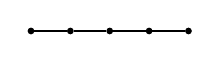
\begin{tikzpicture}[every node/.style={draw, circle, fill=black, minimum size=2pt, inner sep=0pt}]
\node[fill=black] (G1N3) at (5.51,4.51) {};
\node[fill=black] (G1N1) at (6.01,4.51) {};
\node[fill=black] (G1N0) at (6.51,4.51) {};
\node[fill=black] (G1N2) at (7.01,4.51) {};
\node[fill=black] (G1N4) at (7.51,4.51) {};
\draw (G1N0) -- (G1N1);
\draw (G1N0) -- (G1N2);
\draw (G1N1) -- (G1N3);
\draw (G1N2) -- (G1N4);
\end{tikzpicture}
\end{document}
\\  
    \hline
    \end{tabular}

    \vspace{15pt}
%5 vertices
\begin{tabular}{|c|c|c|c|c|c|}
        \hline
        \documentclass{standalone}
\usepackage{tikz}
\begin{document}
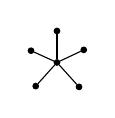
\begin{tikzpicture}[every node/.style={draw, circle, fill=black, minimum size=2pt, inner sep=0pt}]
\node[fill=black] (G1N1) at (6.72,4.69) {};
\node[fill=black] (G1N0) at (6.99,4.99) {};
\node[fill=black] (G1N2) at (7.33,5.15) {};
\node[fill=black] (G1N3) at (7.27,4.68) {};
\node[fill=black] (G1N4) at (6.66,5.14) {};
\node[fill=black] (G1N5) at (6.99,5.39) {};
\draw (G1N0) -- (G1N1);
\draw (G1N0) -- (G1N2);
\draw (G1N0) -- (G1N3);
\draw (G1N0) -- (G1N4);
\draw (G1N0) -- (G1N5);
\end{tikzpicture}
\end{document}
 & \documentclass{standalone}
\usepackage{tikz}
\begin{document}
\begin{tikzpicture}[every node/.style={draw, circle, fill=black, minimum size=2pt, inner sep=0pt}]
\node[fill=black] (G1N2) at (6.00,5.00) {};
\node[fill=black] (G1N0) at (6.50,5.00) {};
\node[fill=black] (G1N1) at (7.00,5.00) {};
\node[fill=black] (G1N5) at (7.50,5.00) {};
\node[fill=black] (G1N3) at (6.50,5.50) {};
\node[fill=black] (G1N4) at (6.50,4.49) {};
\draw (G1N0) -- (G1N1);
\draw (G1N0) -- (G1N2);
\draw (G1N0) -- (G1N3);
\draw (G1N0) -- (G1N4);
\draw (G1N1) -- (G1N5);
\end{tikzpicture}
\end{document}
 & \documentclass{standalone}
\usepackage{tikz}
\begin{document}
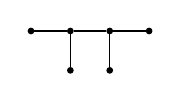
\begin{tikzpicture}[every node/.style={draw, circle, fill=black, minimum size=2pt, inner sep=0pt}]
\node[fill=black] (G1N2) at (5.50,4.51) {};
\node[fill=black] (G1N0) at (6.00,4.51) {};
\node[fill=black] (G1N1) at (6.50,4.51) {};
\node[fill=black] (G1N4) at (7.00,4.51) {};
\node[fill=black] (G1N3) at (6.00,4.01) {};
\node[fill=black] (G1N5) at (6.50,4.01) {};
\draw (G1N0) -- (G1N1);
\draw (G1N0) -- (G1N2);
\draw (G1N0) -- (G1N3);
\draw (G1N1) -- (G1N4);
\draw (G1N1) -- (G1N5);
\end{tikzpicture}
\end{document}
 & \documentclass{standalone}
\usepackage{tikz}
\begin{document}
\begin{tikzpicture}[every node/.style={draw, circle, fill=black, minimum size=2pt, inner sep=0pt}]
\node[fill=black] (G1N4) at (5.50,5.01) {};
\node[fill=black] (G1N1) at (6.00,5.01) {};
\node[fill=black] (G1N0) at (6.50,5.01) {};
\node[fill=black] (G1N2) at (7.00,5.01) {};
\node[fill=black] (G1N5) at (7.50,5.01) {};
\node[fill=black] (G1N3) at (6.50,5.49) {};
\draw (G1N0) -- (G1N1);
\draw (G1N0) -- (G1N2);
\draw (G1N0) -- (G1N3);
\draw (G1N1) -- (G1N4);
\draw (G1N2) -- (G1N5);
\end{tikzpicture}
\end{document}
 & \documentclass{standalone}
\usepackage{tikz}
\begin{document}
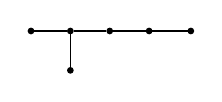
\begin{tikzpicture}[every node/.style={draw, circle, fill=black, minimum size=2pt, inner sep=0pt}]
\node[fill=black] (G1N2) at (5.99,5.01) {};
\node[fill=black] (G1N0) at (6.49,5.01) {};
\node[fill=black] (G1N1) at (6.99,5.01) {};
\node[fill=black] (G1N4) at (7.49,5.01) {};
\node[fill=black] (G1N5) at (8.02,5.01) {};
\node[fill=black] (G1N3) at (6.49,4.51) {};
\draw (G1N0) -- (G1N1);
\draw (G1N0) -- (G1N2);
\draw (G1N0) -- (G1N3);
\draw (G1N1) -- (G1N4);
\draw (G1N4) -- (G1N5);
\end{tikzpicture}
\end{document}
 & \documentclass{standalone}
\usepackage{tikz}
\begin{document}
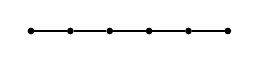
\begin{tikzpicture}[every node/.style={draw, circle, fill=black, minimum size=2pt, inner sep=0pt}]
\node[fill=black] (G1N4) at (5.00,4.51) {};
\node[fill=black] (G1N2) at (5.50,4.51) {};
\node[fill=black] (G1N0) at (6.00,4.51) {};
\node[fill=black] (G1N1) at (6.50,4.51) {};
\node[fill=black] (G1N3) at (7.00,4.51) {};
\node[fill=black] (G1N5) at (7.50,4.51) {};
\draw (G1N0) -- (G1N1);
\draw (G1N0) -- (G1N2);
\draw (G1N1) -- (G1N3);
\draw (G1N2) -- (G1N4);
\draw (G1N3) -- (G1N5);
\end{tikzpicture}
\end{document}
\\ 
        \hline
\end{tabular}

\vspace{15pt}
%6 vertices
\begin{tabular}{|c|c|c|c|c|c|}
    \hline
    \documentclass{standalone}
\usepackage{tikz}
\begin{document}
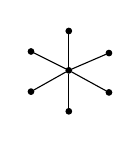
\begin{tikzpicture}[every node/.style={draw, circle, fill=black, minimum size=2pt, inner sep=0pt}]
\node[fill=black] (G1N1) at (6.01,5.24) {};
\node[fill=black] (G1N0) at (6.49,5.00) {};
\node[fill=black] (G1N2) at (7.00,5.22) {};
\node[fill=black] (G1N3) at (6.01,4.73) {};
\node[fill=black] (G1N4) at (7.00,4.72) {};
\node[fill=black] (G1N5) at (6.49,4.48) {};
\node[fill=black] (G1N6) at (6.49,5.50) {};
\draw (G1N0) -- (G1N1);
\draw (G1N0) -- (G1N2);
\draw (G1N0) -- (G1N3);
\draw (G1N0) -- (G1N4);
\draw (G1N0) -- (G1N5);
\draw (G1N0) -- (G1N6);
\end{tikzpicture}
\end{document}
 & \documentclass{standalone}
\usepackage{tikz}
\begin{document}
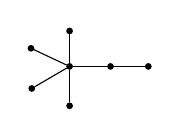
\begin{tikzpicture}[every node/.style={draw, circle, fill=black, minimum size=2pt, inner sep=0pt}]
\node[fill=black] (G1N2) at (6.01,5.22) {};
\node[fill=black] (G1N0) at (6.49,5.50) {};
\node[fill=black] (G1N1) at (7.01,5.50) {};
\node[fill=black] (G1N6) at (7.49,5.50) {};
\node[fill=black] (G1N3) at (6.00,5.73) {};
\node[fill=black] (G1N4) at (6.49,5.00) {};
\node[fill=black] (G1N5) at (6.49,5.95) {};
\draw (G1N0) -- (G1N1);
\draw (G1N0) -- (G1N2);
\draw (G1N0) -- (G1N3);
\draw (G1N0) -- (G1N4);
\draw (G1N0) -- (G1N5);
\draw (G1N1) -- (G1N6);
\end{tikzpicture}
\end{document}
 & \documentclass{standalone}
\usepackage{tikz}
\begin{document}
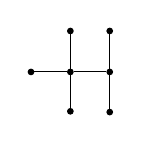
\begin{tikzpicture}[every node/.style={draw, circle, fill=black, minimum size=2pt, inner sep=0pt}]
\node[fill=black] (G1N2) at (6.00,5.50) {};
\node[fill=black] (G1N0) at (6.50,5.50) {};
\node[fill=black] (G1N1) at (7.00,5.50) {};
\node[fill=black] (G1N5) at (7.00,6.02) {};
\node[fill=black] (G1N3) at (6.50,5.00) {};
\node[fill=black] (G1N4) at (6.50,6.02) {};
\node[fill=black] (G1N6) at (7.00,4.99) {};
\draw (G1N0) -- (G1N1);
\draw (G1N0) -- (G1N2);
\draw (G1N0) -- (G1N3);
\draw (G1N0) -- (G1N4);
\draw (G1N1) -- (G1N5);
\draw (G1N1) -- (G1N6);
\end{tikzpicture}
\end{document}
 & \documentclass{standalone}
\usepackage{tikz}
\begin{document}
\begin{tikzpicture}[every node/.style={draw, circle, fill=black, minimum size=2pt, inner sep=0pt}]
\node[fill=black] (G1N5) at (5.49,5.01) {};
\node[fill=black] (G1N1) at (5.99,5.01) {};
\node[fill=black] (G1N0) at (6.49,5.01) {};
\node[fill=black] (G1N2) at (6.99,5.01) {};
\node[fill=black] (G1N6) at (7.49,5.01) {};
\node[fill=black] (G1N3) at (6.49,4.51) {};
\node[fill=black] (G1N4) at (6.49,5.49) {};
\draw (G1N0) -- (G1N1);
\draw (G1N0) -- (G1N2);
\draw (G1N0) -- (G1N3);
\draw (G1N0) -- (G1N4);
\draw (G1N1) -- (G1N5);
\draw (G1N2) -- (G1N6);
\end{tikzpicture}
\end{document}
 & \documentclass{standalone}
\usepackage{tikz}
\begin{document}
\begin{tikzpicture}[every node/.style={draw, circle, fill=black, minimum size=2pt, inner sep=0pt}]
\node[fill=black] (G1N2) at (6.00,5.01) {};
\node[fill=black] (G1N0) at (6.50,5.01) {};
\node[fill=black] (G1N1) at (7.00,5.01) {};
\node[fill=black] (G1N5) at (7.50,5.01) {};
\node[fill=black] (G1N6) at (8.01,5.01) {};
\node[fill=black] (G1N3) at (6.50,4.51) {};
\node[fill=black] (G1N4) at (6.50,5.49) {};
\draw (G1N0) -- (G1N1);
\draw (G1N0) -- (G1N2);
\draw (G1N0) -- (G1N3);
\draw (G1N0) -- (G1N4);
\draw (G1N1) -- (G1N5);
\draw (G1N5) -- (G1N6);
\end{tikzpicture}
\end{document}
 & \documentclass{standalone}
\usepackage{tikz}
\begin{document}
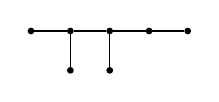
\begin{tikzpicture}[every node/.style={draw, circle, fill=black, minimum size=2pt, inner sep=0pt}]
\node[fill=black] (G1N4) at (5.49,5.01) {};
\node[fill=black] (G1N1) at (5.99,5.01) {};
\node[fill=black] (G1N0) at (6.49,5.01) {};
\node[fill=black] (G1N2) at (6.99,5.01) {};
\node[fill=black] (G1N6) at (7.48,5.01) {};
\node[fill=black] (G1N5) at (5.99,4.51) {};
\node[fill=black] (G1N3) at (6.49,4.51) {};
\draw (G1N0) -- (G1N1);
\draw (G1N0) -- (G1N2);
\draw (G1N0) -- (G1N3);
\draw (G1N1) -- (G1N4);
\draw (G1N1) -- (G1N5);
\draw (G1N2) -- (G1N6);
\end{tikzpicture}
\end{document}
\\ 
    \hline
\end{tabular}

\vspace{1pt}

\begin{tabular}{|c|c|c|c|c|}
    \hline
\documentclass{standalone}
\usepackage{tikz}
\begin{document}
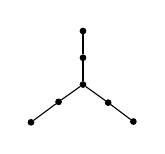
\begin{tikzpicture}[every node/.style={draw, circle, fill=black, minimum size=2pt, inner sep=0pt}]
\node[fill=black] (G1N4) at (5.84,4.53) {};
\node[fill=black] (G1N1) at (6.19,4.79) {};
\node[fill=black] (G1N0) at (6.50,5.01) {};
\node[fill=black] (G1N2) at (6.82,4.78) {};
\node[fill=black] (G1N5) at (7.14,4.54) {};
\node[fill=black] (G1N3) at (6.50,5.35) {};
\node[fill=black] (G1N6) at (6.50,5.69) {};
\draw (G1N0) -- (G1N1);
\draw (G1N0) -- (G1N2);
\draw (G1N0) -- (G1N3);
\draw (G1N1) -- (G1N4);
\draw (G1N2) -- (G1N5);
\draw (G1N3) -- (G1N6);
\end{tikzpicture}
\end{document}
 & \documentclass{standalone}
\usepackage{tikz}
\begin{document}
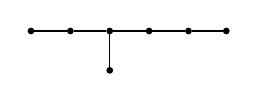
\begin{tikzpicture}[every node/.style={draw, circle, fill=black, minimum size=2pt, inner sep=0pt}]
\node[fill=black] (G1N5) at (5.49,5.00) {};
\node[fill=black] (G1N2) at (5.99,5.00) {};
\node[fill=black] (G1N0) at (6.49,5.00) {};
\node[fill=black] (G1N1) at (6.99,5.00) {};
\node[fill=black] (G1N4) at (7.49,5.00) {};
\node[fill=black] (G1N6) at (7.97,5.00) {};
\node[fill=black] (G1N3) at (6.49,4.50) {};
\draw (G1N0) -- (G1N1);
\draw (G1N0) -- (G1N2);
\draw (G1N0) -- (G1N3);
\draw (G1N1) -- (G1N4);
\draw (G1N2) -- (G1N5);
\draw (G1N4) -- (G1N6);
\end{tikzpicture}
\end{document}
 & \documentclass{standalone}
\usepackage{tikz}
\begin{document}
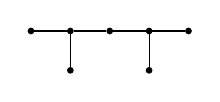
\begin{tikzpicture}[every node/.style={draw, circle, fill=black, minimum size=2pt, inner sep=0pt}]
\node[fill=black] (G1N2) at (5.50,5.00) {};
\node[fill=black] (G1N0) at (6.00,5.00) {};
\node[fill=black] (G1N1) at (6.50,5.00) {};
\node[fill=black] (G1N4) at (7.00,5.00) {};
\node[fill=black] (G1N5) at (7.50,5.00) {};
\node[fill=black] (G1N3) at (6.00,4.50) {};
\node[fill=black] (G1N6) at (7.00,4.50) {};
\draw (G1N0) -- (G1N1);
\draw (G1N0) -- (G1N2);
\draw (G1N0) -- (G1N3);
\draw (G1N1) -- (G1N4);
\draw (G1N4) -- (G1N5);
\draw (G1N4) -- (G1N6);
\end{tikzpicture}
\end{document}
 & \documentclass{standalone}
\usepackage{tikz}
\begin{document}
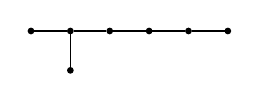
\begin{tikzpicture}[every node/.style={draw, circle, fill=black, minimum size=2pt, inner sep=0pt}]
\node[fill=black] (G1N2) at (5.50,5.00) {};
\node[fill=black] (G1N0) at (6.00,5.00) {};
\node[fill=black] (G1N1) at (6.50,5.00) {};
\node[fill=black] (G1N4) at (7.00,5.00) {};
\node[fill=black] (G1N5) at (7.50,5.00) {};
\node[fill=black] (G1N6) at (8.00,5.00) {};
\node[fill=black] (G1N3) at (6.00,4.50) {};
\draw (G1N0) -- (G1N1);
\draw (G1N0) -- (G1N2);
\draw (G1N0) -- (G1N3);
\draw (G1N1) -- (G1N4);
\draw (G1N4) -- (G1N5);
\draw (G1N5) -- (G1N6);
\end{tikzpicture}
\end{document}
 & \documentclass{standalone}
\usepackage{tikz}
\begin{document}
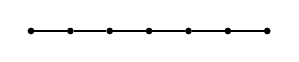
\begin{tikzpicture}[every node/.style={draw, circle, fill=black, minimum size=2pt, inner sep=0pt}]
\node[fill=black] (G1N5) at (5.00,5.01) {};
\node[fill=black] (G1N3) at (5.50,5.01) {};
\node[fill=black] (G1N1) at (6.00,5.01) {};
\node[fill=black] (G1N0) at (6.50,5.01) {};
\node[fill=black] (G1N2) at (7.00,5.01) {};
\node[fill=black] (G1N4) at (7.50,5.01) {};
\node[fill=black] (G1N6) at (8.00,5.01) {};
\draw (G1N0) -- (G1N1);
\draw (G1N0) -- (G1N2);
\draw (G1N1) -- (G1N3);
\draw (G1N2) -- (G1N4);
\draw (G1N3) -- (G1N5);
\draw (G1N4) -- (G1N6);
\end{tikzpicture}
\end{document}
 \\
    \hline
\end{tabular}

\vspace{5pt}
OR

% Globally set minimum row height and padding
\renewcommand{\arraystretch}{1.5}  % Adjusts the vertical space between rows (default is 1)

% Set vertical padding with \extrarowheight
\setlength{\extrarowheight}{20pt}  % Adds extra vertical space between rows

% Set horizontal padding (already done for you)
\setlength{\tabcolsep}{12pt}  % Adjust horizontal cell padding

% Set table border thickness (optional)
\setlength{\arrayrulewidth}{0.5mm}  % Set border thickness
\begin{tabular}{|c|c|c|c|c|c|}
    \hline
    \documentclass{standalone}
\usepackage{tikz}
\begin{document}
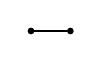
\begin{tikzpicture}[every node/.style={draw, circle, fill=black, minimum size=2pt, inner sep=0pt}]
\node[fill=black] (G1N0) at (6.50,4.50) {};
\node[fill=black] (G1N1) at (7.00,4.50) {};
\draw (G1N0) -- (G1N1);
\end{tikzpicture}
\end{document}
 & \documentclass{standalone}
\usepackage{tikz}
\begin{document}
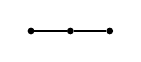
\begin{tikzpicture}[every node/.style={draw, circle, fill=black, minimum size=2pt, inner sep=0pt}]
\node[fill=black] (G1N1) at (5.99,4.51) {};
\node[fill=black] (G1N0) at (6.49,4.51) {};
\node[fill=black] (G1N2) at (6.99,4.51) {};
\draw (G1N0) -- (G1N1);
\draw (G1N0) -- (G1N2);
\end{tikzpicture}
\end{document}
 & \documentclass{standalone}
\usepackage{tikz}
\begin{document}
\begin{tikzpicture}[every node/.style={draw, circle, fill=black, minimum size=2pt, inner sep=0pt}]
\node[fill=black] (G1N1) at (6.00,4.50) {};
\node[fill=black] (G1N0) at (6.50,4.50) {};
\node[fill=black] (G1N2) at (7.00,4.50) {};
\node[fill=black] (G1N3) at (6.50,4.99) {};
\draw (G1N0) -- (G1N1);
\draw (G1N0) -- (G1N2);
\draw (G1N0) -- (G1N3);
\end{tikzpicture}
\end{document}
 & \documentclass{standalone}
\usepackage{tikz}
\begin{document}
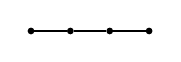
\begin{tikzpicture}[every node/.style={draw, circle, fill=black, minimum size=2pt, inner sep=0pt}]
\node[fill=black] (G1N2) at (6.00,4.50) {};
\node[fill=black] (G1N0) at (6.50,4.50) {};
\node[fill=black] (G1N1) at (7.00,4.50) {};
\node[fill=black] (G1N3) at (7.50,4.50) {};
\draw (G1N0) -- (G1N1);
\draw (G1N0) -- (G1N2);
\draw (G1N1) -- (G1N3);
\end{tikzpicture}
\end{document}
 \\ 
    \hline
    \documentclass{standalone}
\usepackage{tikz}
\begin{document}
\begin{tikzpicture}[every node/.style={draw, circle, fill=black, minimum size=2pt, inner sep=0pt}]
\node[fill=black] (G1N1) at (6.00,4.51) {};
\node[fill=black] (G1N0) at (6.50,4.51) {};
\node[fill=black] (G1N2) at (7.00,4.51) {};
\node[fill=black] (G1N3) at (6.50,4.01) {};
\node[fill=black] (G1N4) at (6.50,5.00) {};
\draw (G1N0) -- (G1N1);
\draw (G1N0) -- (G1N2);
\draw (G1N0) -- (G1N3);
\draw (G1N0) -- (G1N4);
\end{tikzpicture}
\end{document}
 & \documentclass{standalone}
\usepackage{tikz}
\begin{document}
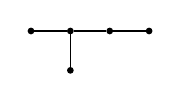
\begin{tikzpicture}[every node/.style={draw, circle, fill=black, minimum size=2pt, inner sep=0pt}]
\node[fill=black] (G1N2) at (6.00,4.50) {};
\node[fill=black] (G1N0) at (6.50,4.50) {};
\node[fill=black] (G1N1) at (7.00,4.50) {};
\node[fill=black] (G1N4) at (7.50,4.50) {};
\node[fill=black] (G1N3) at (6.50,4.00) {};
\draw (G1N0) -- (G1N1);
\draw (G1N0) -- (G1N2);
\draw (G1N0) -- (G1N3);
\draw (G1N1) -- (G1N4);
\end{tikzpicture}
\end{document}
 & \documentclass{standalone}
\usepackage{tikz}
\begin{document}
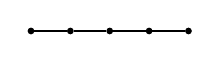
\begin{tikzpicture}[every node/.style={draw, circle, fill=black, minimum size=2pt, inner sep=0pt}]
\node[fill=black] (G1N3) at (5.51,4.51) {};
\node[fill=black] (G1N1) at (6.01,4.51) {};
\node[fill=black] (G1N0) at (6.51,4.51) {};
\node[fill=black] (G1N2) at (7.01,4.51) {};
\node[fill=black] (G1N4) at (7.51,4.51) {};
\draw (G1N0) -- (G1N1);
\draw (G1N0) -- (G1N2);
\draw (G1N1) -- (G1N3);
\draw (G1N2) -- (G1N4);
\end{tikzpicture}
\end{document}
 & \documentclass{standalone}
\usepackage{tikz}
\begin{document}
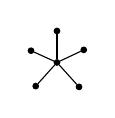
\begin{tikzpicture}[every node/.style={draw, circle, fill=black, minimum size=2pt, inner sep=0pt}]
\node[fill=black] (G1N1) at (6.72,4.69) {};
\node[fill=black] (G1N0) at (6.99,4.99) {};
\node[fill=black] (G1N2) at (7.33,5.15) {};
\node[fill=black] (G1N3) at (7.27,4.68) {};
\node[fill=black] (G1N4) at (6.66,5.14) {};
\node[fill=black] (G1N5) at (6.99,5.39) {};
\draw (G1N0) -- (G1N1);
\draw (G1N0) -- (G1N2);
\draw (G1N0) -- (G1N3);
\draw (G1N0) -- (G1N4);
\draw (G1N0) -- (G1N5);
\end{tikzpicture}
\end{document}
 \\
    \hline
    \documentclass{standalone}
\usepackage{tikz}
\begin{document}
\begin{tikzpicture}[every node/.style={draw, circle, fill=black, minimum size=2pt, inner sep=0pt}]
\node[fill=black] (G1N2) at (6.00,5.00) {};
\node[fill=black] (G1N0) at (6.50,5.00) {};
\node[fill=black] (G1N1) at (7.00,5.00) {};
\node[fill=black] (G1N5) at (7.50,5.00) {};
\node[fill=black] (G1N3) at (6.50,5.50) {};
\node[fill=black] (G1N4) at (6.50,4.49) {};
\draw (G1N0) -- (G1N1);
\draw (G1N0) -- (G1N2);
\draw (G1N0) -- (G1N3);
\draw (G1N0) -- (G1N4);
\draw (G1N1) -- (G1N5);
\end{tikzpicture}
\end{document}
 & \documentclass{standalone}
\usepackage{tikz}
\begin{document}
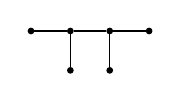
\begin{tikzpicture}[every node/.style={draw, circle, fill=black, minimum size=2pt, inner sep=0pt}]
\node[fill=black] (G1N2) at (5.50,4.51) {};
\node[fill=black] (G1N0) at (6.00,4.51) {};
\node[fill=black] (G1N1) at (6.50,4.51) {};
\node[fill=black] (G1N4) at (7.00,4.51) {};
\node[fill=black] (G1N3) at (6.00,4.01) {};
\node[fill=black] (G1N5) at (6.50,4.01) {};
\draw (G1N0) -- (G1N1);
\draw (G1N0) -- (G1N2);
\draw (G1N0) -- (G1N3);
\draw (G1N1) -- (G1N4);
\draw (G1N1) -- (G1N5);
\end{tikzpicture}
\end{document}
 & \documentclass{standalone}
\usepackage{tikz}
\begin{document}
\begin{tikzpicture}[every node/.style={draw, circle, fill=black, minimum size=2pt, inner sep=0pt}]
\node[fill=black] (G1N4) at (5.50,5.01) {};
\node[fill=black] (G1N1) at (6.00,5.01) {};
\node[fill=black] (G1N0) at (6.50,5.01) {};
\node[fill=black] (G1N2) at (7.00,5.01) {};
\node[fill=black] (G1N5) at (7.50,5.01) {};
\node[fill=black] (G1N3) at (6.50,5.49) {};
\draw (G1N0) -- (G1N1);
\draw (G1N0) -- (G1N2);
\draw (G1N0) -- (G1N3);
\draw (G1N1) -- (G1N4);
\draw (G1N2) -- (G1N5);
\end{tikzpicture}
\end{document}
 & \documentclass{standalone}
\usepackage{tikz}
\begin{document}
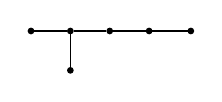
\begin{tikzpicture}[every node/.style={draw, circle, fill=black, minimum size=2pt, inner sep=0pt}]
\node[fill=black] (G1N2) at (5.99,5.01) {};
\node[fill=black] (G1N0) at (6.49,5.01) {};
\node[fill=black] (G1N1) at (6.99,5.01) {};
\node[fill=black] (G1N4) at (7.49,5.01) {};
\node[fill=black] (G1N5) at (8.02,5.01) {};
\node[fill=black] (G1N3) at (6.49,4.51) {};
\draw (G1N0) -- (G1N1);
\draw (G1N0) -- (G1N2);
\draw (G1N0) -- (G1N3);
\draw (G1N1) -- (G1N4);
\draw (G1N4) -- (G1N5);
\end{tikzpicture}
\end{document}
 \\
    \hline
    \documentclass{standalone}
\usepackage{tikz}
\begin{document}
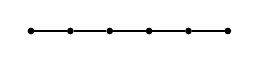
\begin{tikzpicture}[every node/.style={draw, circle, fill=black, minimum size=2pt, inner sep=0pt}]
\node[fill=black] (G1N4) at (5.00,4.51) {};
\node[fill=black] (G1N2) at (5.50,4.51) {};
\node[fill=black] (G1N0) at (6.00,4.51) {};
\node[fill=black] (G1N1) at (6.50,4.51) {};
\node[fill=black] (G1N3) at (7.00,4.51) {};
\node[fill=black] (G1N5) at (7.50,4.51) {};
\draw (G1N0) -- (G1N1);
\draw (G1N0) -- (G1N2);
\draw (G1N1) -- (G1N3);
\draw (G1N2) -- (G1N4);
\draw (G1N3) -- (G1N5);
\end{tikzpicture}
\end{document}
 & \documentclass{standalone}
\usepackage{tikz}
\begin{document}
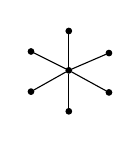
\begin{tikzpicture}[every node/.style={draw, circle, fill=black, minimum size=2pt, inner sep=0pt}]
\node[fill=black] (G1N1) at (6.01,5.24) {};
\node[fill=black] (G1N0) at (6.49,5.00) {};
\node[fill=black] (G1N2) at (7.00,5.22) {};
\node[fill=black] (G1N3) at (6.01,4.73) {};
\node[fill=black] (G1N4) at (7.00,4.72) {};
\node[fill=black] (G1N5) at (6.49,4.48) {};
\node[fill=black] (G1N6) at (6.49,5.50) {};
\draw (G1N0) -- (G1N1);
\draw (G1N0) -- (G1N2);
\draw (G1N0) -- (G1N3);
\draw (G1N0) -- (G1N4);
\draw (G1N0) -- (G1N5);
\draw (G1N0) -- (G1N6);
\end{tikzpicture}
\end{document}
 & \documentclass{standalone}
\usepackage{tikz}
\begin{document}
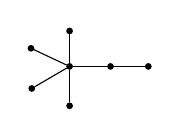
\begin{tikzpicture}[every node/.style={draw, circle, fill=black, minimum size=2pt, inner sep=0pt}]
\node[fill=black] (G1N2) at (6.01,5.22) {};
\node[fill=black] (G1N0) at (6.49,5.50) {};
\node[fill=black] (G1N1) at (7.01,5.50) {};
\node[fill=black] (G1N6) at (7.49,5.50) {};
\node[fill=black] (G1N3) at (6.00,5.73) {};
\node[fill=black] (G1N4) at (6.49,5.00) {};
\node[fill=black] (G1N5) at (6.49,5.95) {};
\draw (G1N0) -- (G1N1);
\draw (G1N0) -- (G1N2);
\draw (G1N0) -- (G1N3);
\draw (G1N0) -- (G1N4);
\draw (G1N0) -- (G1N5);
\draw (G1N1) -- (G1N6);
\end{tikzpicture}
\end{document}
 & \documentclass{standalone}
\usepackage{tikz}
\begin{document}
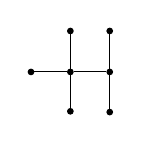
\begin{tikzpicture}[every node/.style={draw, circle, fill=black, minimum size=2pt, inner sep=0pt}]
\node[fill=black] (G1N2) at (6.00,5.50) {};
\node[fill=black] (G1N0) at (6.50,5.50) {};
\node[fill=black] (G1N1) at (7.00,5.50) {};
\node[fill=black] (G1N5) at (7.00,6.02) {};
\node[fill=black] (G1N3) at (6.50,5.00) {};
\node[fill=black] (G1N4) at (6.50,6.02) {};
\node[fill=black] (G1N6) at (7.00,4.99) {};
\draw (G1N0) -- (G1N1);
\draw (G1N0) -- (G1N2);
\draw (G1N0) -- (G1N3);
\draw (G1N0) -- (G1N4);
\draw (G1N1) -- (G1N5);
\draw (G1N1) -- (G1N6);
\end{tikzpicture}
\end{document}
 \\
    \hline
    \documentclass{standalone}
\usepackage{tikz}
\begin{document}
\begin{tikzpicture}[every node/.style={draw, circle, fill=black, minimum size=2pt, inner sep=0pt}]
\node[fill=black] (G1N5) at (5.49,5.01) {};
\node[fill=black] (G1N1) at (5.99,5.01) {};
\node[fill=black] (G1N0) at (6.49,5.01) {};
\node[fill=black] (G1N2) at (6.99,5.01) {};
\node[fill=black] (G1N6) at (7.49,5.01) {};
\node[fill=black] (G1N3) at (6.49,4.51) {};
\node[fill=black] (G1N4) at (6.49,5.49) {};
\draw (G1N0) -- (G1N1);
\draw (G1N0) -- (G1N2);
\draw (G1N0) -- (G1N3);
\draw (G1N0) -- (G1N4);
\draw (G1N1) -- (G1N5);
\draw (G1N2) -- (G1N6);
\end{tikzpicture}
\end{document}
 & \documentclass{standalone}
\usepackage{tikz}
\begin{document}
\begin{tikzpicture}[every node/.style={draw, circle, fill=black, minimum size=2pt, inner sep=0pt}]
\node[fill=black] (G1N2) at (6.00,5.01) {};
\node[fill=black] (G1N0) at (6.50,5.01) {};
\node[fill=black] (G1N1) at (7.00,5.01) {};
\node[fill=black] (G1N5) at (7.50,5.01) {};
\node[fill=black] (G1N6) at (8.01,5.01) {};
\node[fill=black] (G1N3) at (6.50,4.51) {};
\node[fill=black] (G1N4) at (6.50,5.49) {};
\draw (G1N0) -- (G1N1);
\draw (G1N0) -- (G1N2);
\draw (G1N0) -- (G1N3);
\draw (G1N0) -- (G1N4);
\draw (G1N1) -- (G1N5);
\draw (G1N5) -- (G1N6);
\end{tikzpicture}
\end{document}
 & \documentclass{standalone}
\usepackage{tikz}
\begin{document}
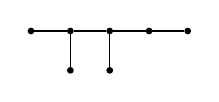
\begin{tikzpicture}[every node/.style={draw, circle, fill=black, minimum size=2pt, inner sep=0pt}]
\node[fill=black] (G1N4) at (5.49,5.01) {};
\node[fill=black] (G1N1) at (5.99,5.01) {};
\node[fill=black] (G1N0) at (6.49,5.01) {};
\node[fill=black] (G1N2) at (6.99,5.01) {};
\node[fill=black] (G1N6) at (7.48,5.01) {};
\node[fill=black] (G1N5) at (5.99,4.51) {};
\node[fill=black] (G1N3) at (6.49,4.51) {};
\draw (G1N0) -- (G1N1);
\draw (G1N0) -- (G1N2);
\draw (G1N0) -- (G1N3);
\draw (G1N1) -- (G1N4);
\draw (G1N1) -- (G1N5);
\draw (G1N2) -- (G1N6);
\end{tikzpicture}
\end{document}
 & \documentclass{standalone}
\usepackage{tikz}
\begin{document}
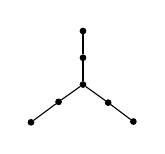
\begin{tikzpicture}[every node/.style={draw, circle, fill=black, minimum size=2pt, inner sep=0pt}]
\node[fill=black] (G1N4) at (5.84,4.53) {};
\node[fill=black] (G1N1) at (6.19,4.79) {};
\node[fill=black] (G1N0) at (6.50,5.01) {};
\node[fill=black] (G1N2) at (6.82,4.78) {};
\node[fill=black] (G1N5) at (7.14,4.54) {};
\node[fill=black] (G1N3) at (6.50,5.35) {};
\node[fill=black] (G1N6) at (6.50,5.69) {};
\draw (G1N0) -- (G1N1);
\draw (G1N0) -- (G1N2);
\draw (G1N0) -- (G1N3);
\draw (G1N1) -- (G1N4);
\draw (G1N2) -- (G1N5);
\draw (G1N3) -- (G1N6);
\end{tikzpicture}
\end{document}
 \\
    \hline
    \documentclass{standalone}
\usepackage{tikz}
\begin{document}
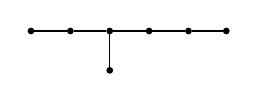
\begin{tikzpicture}[every node/.style={draw, circle, fill=black, minimum size=2pt, inner sep=0pt}]
\node[fill=black] (G1N5) at (5.49,5.00) {};
\node[fill=black] (G1N2) at (5.99,5.00) {};
\node[fill=black] (G1N0) at (6.49,5.00) {};
\node[fill=black] (G1N1) at (6.99,5.00) {};
\node[fill=black] (G1N4) at (7.49,5.00) {};
\node[fill=black] (G1N6) at (7.97,5.00) {};
\node[fill=black] (G1N3) at (6.49,4.50) {};
\draw (G1N0) -- (G1N1);
\draw (G1N0) -- (G1N2);
\draw (G1N0) -- (G1N3);
\draw (G1N1) -- (G1N4);
\draw (G1N2) -- (G1N5);
\draw (G1N4) -- (G1N6);
\end{tikzpicture}
\end{document}
 & \documentclass{standalone}
\usepackage{tikz}
\begin{document}
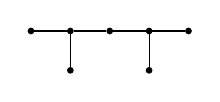
\begin{tikzpicture}[every node/.style={draw, circle, fill=black, minimum size=2pt, inner sep=0pt}]
\node[fill=black] (G1N2) at (5.50,5.00) {};
\node[fill=black] (G1N0) at (6.00,5.00) {};
\node[fill=black] (G1N1) at (6.50,5.00) {};
\node[fill=black] (G1N4) at (7.00,5.00) {};
\node[fill=black] (G1N5) at (7.50,5.00) {};
\node[fill=black] (G1N3) at (6.00,4.50) {};
\node[fill=black] (G1N6) at (7.00,4.50) {};
\draw (G1N0) -- (G1N1);
\draw (G1N0) -- (G1N2);
\draw (G1N0) -- (G1N3);
\draw (G1N1) -- (G1N4);
\draw (G1N4) -- (G1N5);
\draw (G1N4) -- (G1N6);
\end{tikzpicture}
\end{document}
 & \documentclass{standalone}
\usepackage{tikz}
\begin{document}
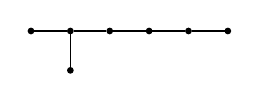
\begin{tikzpicture}[every node/.style={draw, circle, fill=black, minimum size=2pt, inner sep=0pt}]
\node[fill=black] (G1N2) at (5.50,5.00) {};
\node[fill=black] (G1N0) at (6.00,5.00) {};
\node[fill=black] (G1N1) at (6.50,5.00) {};
\node[fill=black] (G1N4) at (7.00,5.00) {};
\node[fill=black] (G1N5) at (7.50,5.00) {};
\node[fill=black] (G1N6) at (8.00,5.00) {};
\node[fill=black] (G1N3) at (6.00,4.50) {};
\draw (G1N0) -- (G1N1);
\draw (G1N0) -- (G1N2);
\draw (G1N0) -- (G1N3);
\draw (G1N1) -- (G1N4);
\draw (G1N4) -- (G1N5);
\draw (G1N5) -- (G1N6);
\end{tikzpicture}
\end{document}
 & \documentclass{standalone}
\usepackage{tikz}
\begin{document}
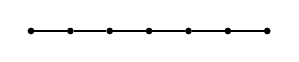
\begin{tikzpicture}[every node/.style={draw, circle, fill=black, minimum size=2pt, inner sep=0pt}]
\node[fill=black] (G1N5) at (5.00,5.01) {};
\node[fill=black] (G1N3) at (5.50,5.01) {};
\node[fill=black] (G1N1) at (6.00,5.01) {};
\node[fill=black] (G1N0) at (6.50,5.01) {};
\node[fill=black] (G1N2) at (7.00,5.01) {};
\node[fill=black] (G1N4) at (7.50,5.01) {};
\node[fill=black] (G1N6) at (8.00,5.01) {};
\draw (G1N0) -- (G1N1);
\draw (G1N0) -- (G1N2);
\draw (G1N1) -- (G1N3);
\draw (G1N2) -- (G1N4);
\draw (G1N3) -- (G1N5);
\draw (G1N4) -- (G1N6);
\end{tikzpicture}
\end{document}
\\
    \hline
\end{tabular}

\end{document}
